% !TeX spellcheck = en_US
\newpage
\section{Network types}
\subsection{CDN}
\begin{wrapfigure}[11]{r}{5cm}
	\vspace{-1cm}
	\begin{center}
		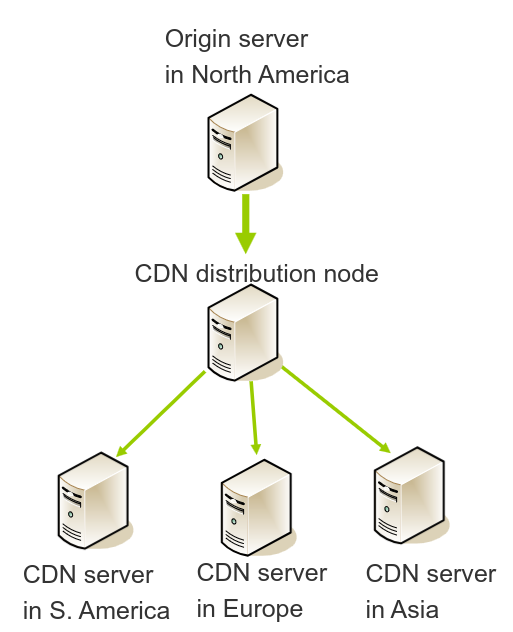
\includegraphics[width=5cm]{cdn}
	\end{center}
\end{wrapfigure}
\textbf{Content Delivery Networks} help to scale many distributed web requests (e.g. video streaming, drive). The principle is similar to DNS caches: the shared content is replicated everywhere and you access a close-by one instead of the central server.
\subsubsection{How}
Content replication can be done with two different strategies (often used at the same time):
\begin{itemize}
	\item \textbf{PULL}: the first request will have to fetch the data from the central server and replicate it locally, when the cache is full erase recently least used content
	\item \textbf{PUSH}: content expected to be popular can be pre-provisioned in caches
\end{itemize}
Then, \textbf{DNS CNAME} feature is used to redirect hosts to the nearest cache server since the name resolution is done based on geographical position.
\begin{center}
	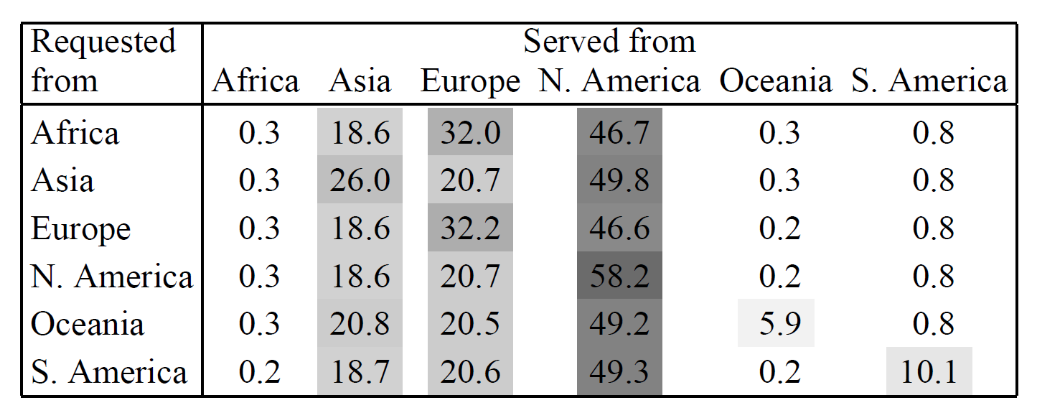
\includegraphics[scale=.3]{dnsredir}
\end{center}

\subsubsection{Where}
The service of a CDN company is to deliver the content fast. There are basically two design principles:
\begin{itemize}
	\item \textbf{On-net}: deploy CDN servers directly into ISP points of presence, hence getting very close to the end-user but becoming complex to maintain the shuffling of content since they are scattered among different AS
	\item \textbf{Off-net}: connect few CDN data centers to ISPs, hence less maintenance but dependence from ISP POPs and a bit higher delays
\end{itemize}

\subsubsection{Hypergiants}
Hypergiants are large content providers, cloud providers and CDNs that are typically responsible for distributing the majority of traffic to the end user (e.g. Google, Netflix, Meta).\\
They reshape the internet by improving capacity, latency and congestion.

\subsubsection{Advantages}
The advantages of CDNs are:
\begin{itemize}
	\item \textbf{Robustness}: so many caches that you can't do a DoS attack
	\item \textbf{Scalability}: load is spread to thousands of servers
	\item \textbf{Lower latency}: content is accessed from a local cache
\end{itemize}
The main \textbf{disadvantage} is that it makes the internet and the services much more complex.

\subsection{ICN}
\textbf{Information Centric Networking} allows for improved \textbf{security} and more \textbf{efficient content distribution}. It's based on the principle to request access for the content and not the node, in a publish/subscribe paradigm: we address the content by a name, which is augmented with authentication. All of this with a lot of caching.\\\\

The content provider places the resource in a shared server. Then the customer specifies an \textbf{interest} to that object, which is store in the routers in a \textbf{Pending Interest Table}. Then the interest gets forwarded using the data in the \textbf{Forwarding Information Base} until it finds the requested resource, which gets back and gets cached along the way.

\begin{center}
	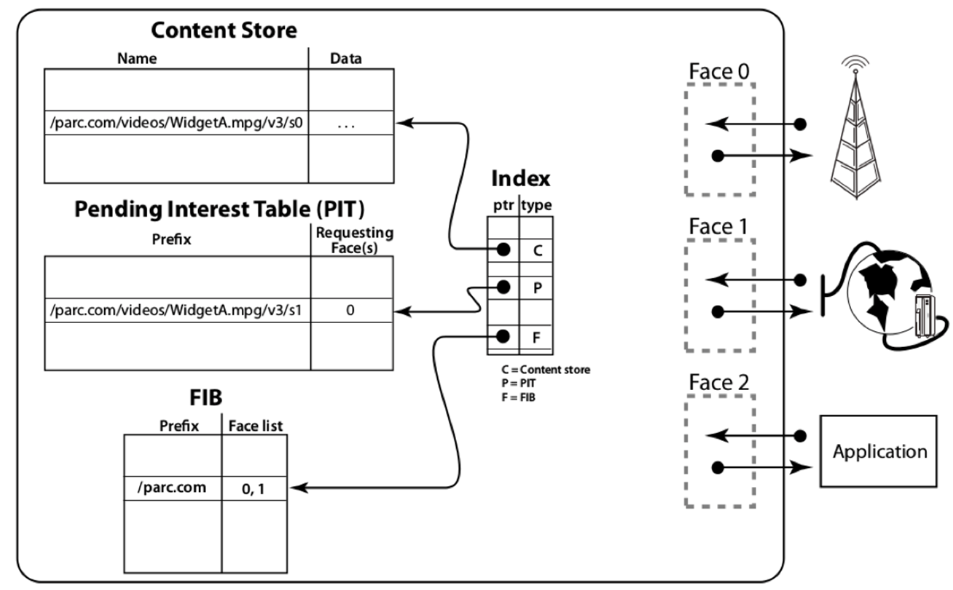
\includegraphics[scale=.3]{icnnode}
\end{center}

\subsubsection{NDN}
\textbf{Named Data Networking} is one way to implement an ICN.
\begin{center}
	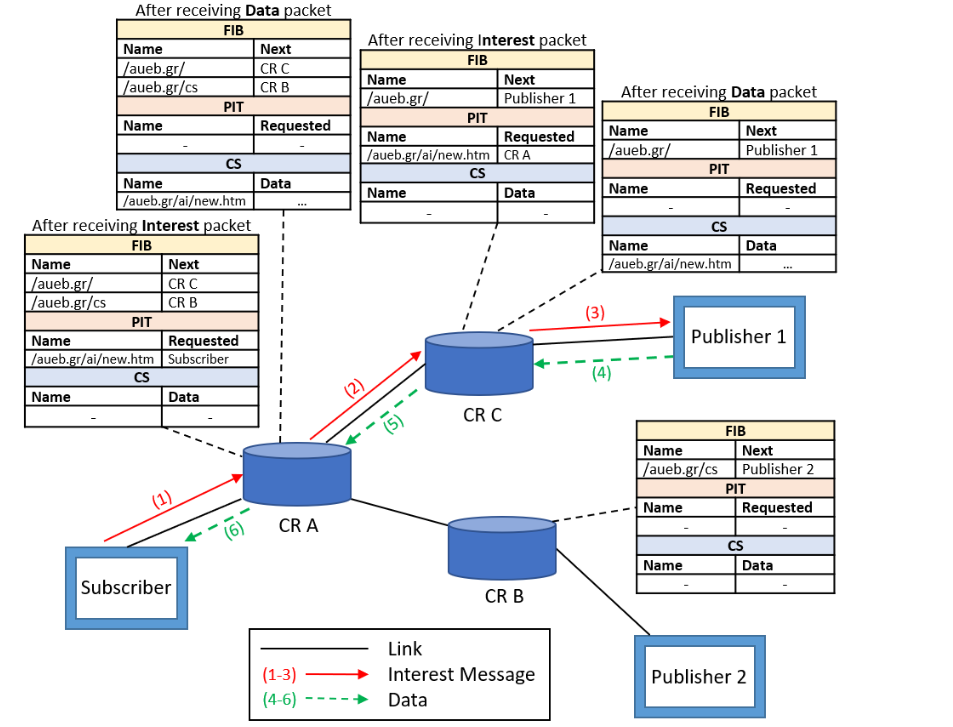
\includegraphics[scale=.4]{ndn}
\end{center}
\textbf{SAIL} is another implementation of an ICN that uses both regular routing techniques and Name-Based.

\subsection{P2P}
In a \textbf{Peer-To-Peer} architecture each member of the network is both client and server and it's called \textbf{peer}. They operate at the application layer. The main advantages are:
\begin{itemize}
	\item No central entity, no single point of failure
	\item Reduces/eliminates the demand for server clusters
	\item Content replication
	\item Flexibility, self-organization
	\item Some levels of anonymity
	\item Efficiency
\end{itemize}

\subsubsection{Unstructured}
An unstructured P2P network has data placed \textbf{randomly}. Then decentralized \textbf{flooding} is used to spread it around the network, up to having it replicated on all peers.\\
The more data we have flooded, the less there is a need for central servers, but at the same time that increases \textbf{communication overhead}.
\begin{center}
	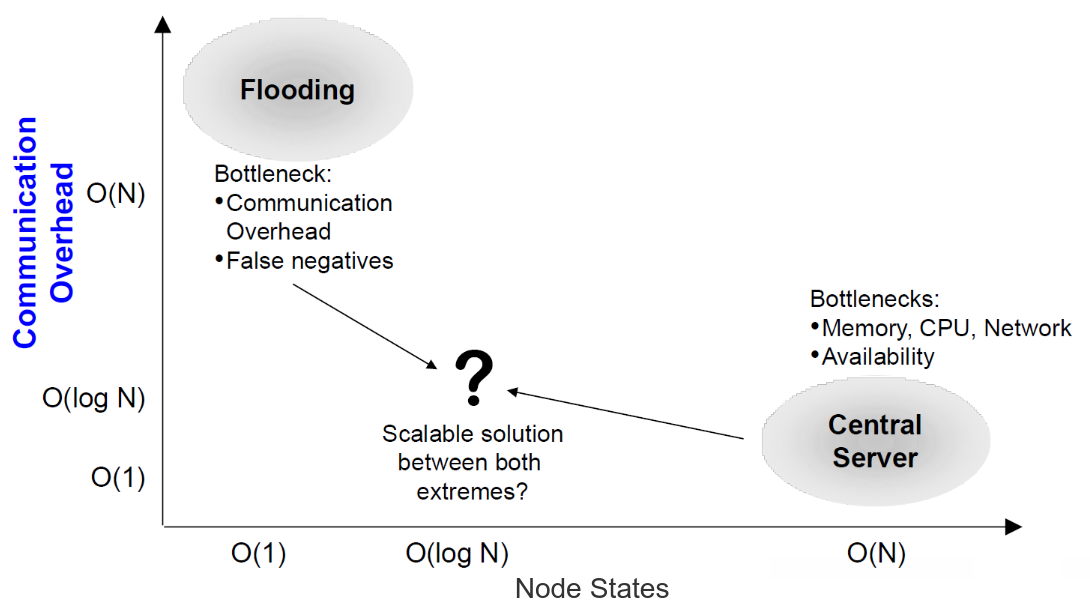
\includegraphics[scale=.3]{p2puns}
\end{center}

\subsubsection{Structured}
In a structured P2P data is placed \textbf{systematically} and there is a systematic overlay routing. The main challenge is where to store and how to find a certain item without any centralized control or coordination.\\\\
There are two \textbf{lookup} approaches:
\begin{itemize}
	\item \textbf{Centralized}: using a server
	\item \textbf{Distributed}: using \textbf{Distributed Hash Tables}
\end{itemize}

\paragraph{DHT}
In a DHT nodes are structured according to some flat address space and are responsible for data in a certain part of it. Intermediate nodes maintain routing information to target nodes.\\\\
Each node manages a small number of references to other nodes and the data itself and needs only a small number ($O(\log N)$) of routing steps to reach the destination. Identifiers are distributed on the nodes nearly equally, hence balancing the load among them.

There are multiple algorithms to achieve this type of data structuring (Chord, Tapestry, Content Addressable Network). An example is \textbf{Pastry}: nodes are organized in a virtual ID ring from $0$ to $2^{128}-1$ and to each node and object a $128$bit hash key is assigned.\\
The routing is based on \textit{longest prefix matching} considering the topological distance: each node maintains a forwarding table and a leaf set. Leaf sets provides shortcuts: contains the $L$ closest nodes, $\frac{L}{2}$ smaller nodes by ID and $\frac{L}{2}$ larger nodes by ID, with $\lvert L \rvert$ usually being $2^b$ or $2 \cdot 2^b$.
\begin{enumerate}
	\item Node $n$ searches the node responsible for key $k$
	\item $n$ searches its forwarding table for a node with a better prefix matching (at least one or more digits matching $k$)
	\item If such a node does not exist the leaf set is searched for a node which is lexicographically closer to $k$
	\item Repeat in each node until found ($O(\log_2^b N)$)
\end{enumerate}

\begin{wrapfigure}[7]{r}{3.5cm}
	\vspace{-1cm}
	\begin{center}
		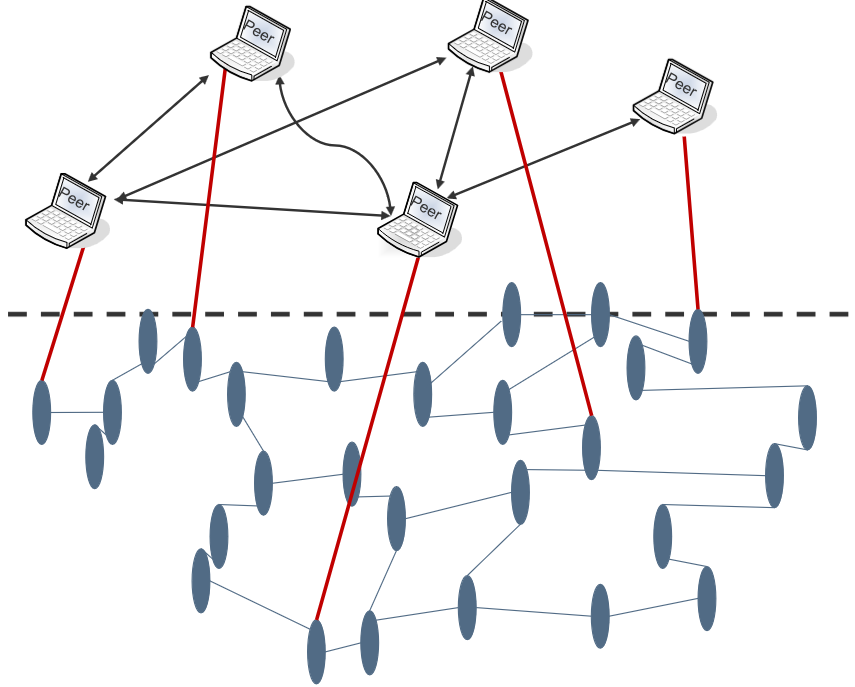
\includegraphics[width=3.5cm]{p2poverlay}
	\end{center}
\end{wrapfigure}
DHTs can route very efficiently on the \textbf{overlay network}, however there is no relationship between that and the physical topology.\\\\
In fact, neighbors on one may not be neighbors in the other, hence causing an \textbf{overlay stretch}: the ratio between the accumulated physical routes during the overlay routing and the real path.
\begin{center}
	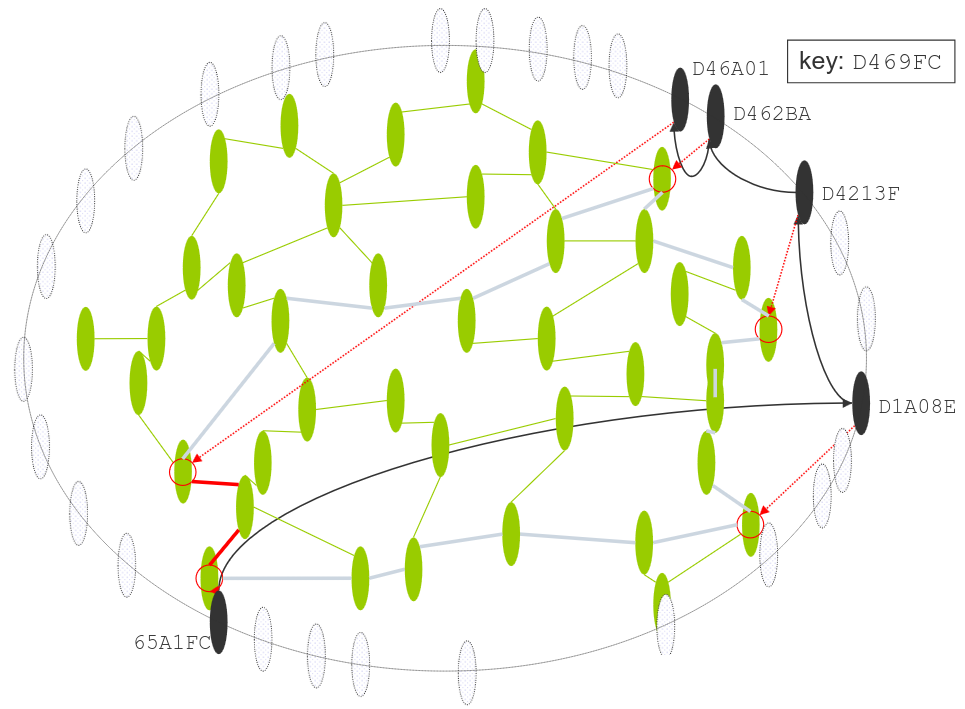
\includegraphics[scale=.3]{overstretch}
\end{center}
There are several method to reduce this phenomena, such as \textbf{Proximity Node Selection}: each node selects periodically a random entry from its routing table at row $i$. This node then replies with his $i$-th entry. After the response, the second node compares the distance  between the own entries and the response and if physically closer it replaces it.\\\\
Another approach is the \textbf{landmarking}: a fixed set of nodes are set as landmarks; periodically each nodes compute their distance from them and nodes with the same one assign each other numerical close overlay IDs.